\documentclass[12pt]{article}
\usepackage{fullpage}
\usepackage{multicol}
\usepackage{graphicx}
\usepackage{fontspec}
\setmainfont{OpenDyslexicAlta}
\newcommand{\blk}{\underline{\hspace{0.5in}}}
\begin{document}
%\maketitle
\center{\section*{Geometry Test 1}}
\center{\section*{Work in your NOTEBOOK!}}
%\begin{multicols}{2}
\begin{enumerate}
	\item Evaluate:
	\begin{enumerate}
		%\item $3\cdot 4$
		%\item $12 - 7$
		\item $7 - 12$
		\item $4^2$
		\item $7-2\cdot 3$
		\item $4\cdot(7-2)$
		\item $6- 8/2$
	\end{enumerate}
	\item Substitute $x=2, y=-12, z=4$ into the expression $xy - z$.
	\item Compare the following decimals with $<, >$ or$ =$:
	\begin{enumerate}
		\item $0.5 \blk{} 0.4$
		\item $0.415 \blk 0.5$
		%\item $9.9 \blk 10.01$
		%		\item $1.3 \blk -5.9$
		\item $3.131000 \blk 3.131$
	\end{enumerate}
	\item Evaluate:
	\begin{enumerate}
		\item $3.4 + 5.2$
		%		\item $3.3 + 2.9$
		\item $2.4 + 3.815$
		\item $9.6 - 3.7$
		%\item $9.7 - 3.52$
		%		\item $2.9 - 25$
		%		\item $4 \cdot 3.6 - 5.1$
		\item $15.4 \div 4$
	\end{enumerate}
	\item Substitute $x=1.6, y=-4.2$ into $xy$.
	\item Write in scientific notation:
	\begin{enumerate}
		\item $54000$
		\item $514$
		\item $0.0054$
		%\item $-0.015$
	\end{enumerate}
	\item Write each number as a decimal number
	\begin{enumerate}
		\item $6.7 \times 10^3$
		\item $5.14 \times 10^{-3}$
	\end{enumerate}
	\item Add or subtract the following fractions
	\begin{enumerate}
		\item $\frac{1}{5} + \frac{3}{5}$
		\item $\frac{1}{4} + \frac{1}{5}$
		\item $\frac{7}{3} - \frac{3}{4}$
		%		\item $\frac{7}{8} - \frac{1}{2}$
	\end{enumerate}
	\item Compare the fractions using $<, >$ and $=$:
	\begin{enumerate}
		\item $\frac{2}{7} \blk \frac{1}{7}$
		\item $\frac{-8}{9} \blk \frac{2}{9}$ 
		\item $\frac{3}{5} \blk \frac{4}{7}$
		%\item $\frac{2}{3} \blk \frac{6}{9}$
	\end{enumerate}
	\item Simplify the following fractions:
	\begin{enumerate}
		\item $\frac{3}{6}$
		\item $\frac{10}{18}$
		\item $\frac{10x^2}{18x^4}$
	\end{enumerate}
	\item Convert the $\frac{3}{7}$ to a decimal.
	\item Convert the $0.73$ to a fraction.
	\item Perform the indicated operations:
	\begin{enumerate}
		\item $\frac{3}{7} \cdot \frac{4}{5}$
		\item $\frac{4}{5} \div \frac{1}{3}$
	\end{enumerate}
	\item Illustrate each of the following by labeling two points P and T and drawing the picture:
	\begin{enumerate}
		\item $R_{TP}$
%		\item $R_{PT}$
		\item $\overline{TP}$
		\item $L_{TP}$
	\end{enumerate}
	\item Construct a triangle whose sides are length 3 cm, 5 cm, and 6 cm.  What are the angles of that triangle.
%	\item In the picture below of the Earth, the $Point$ is at latitude $40^o$ North.  If the circumference of the Earth is 36000km, how far is the Point from the equator?
%
%	\includegraphics*[width=3in]{latitude.png}
\item There are $360^o$ longitude on the earth.  How long is one degree if the circumference of the earth is 24,000 mile?
\item What is the definition of supplementary angles?

	\item We have 2 points $X$ and $Y$ that are both less than 8 cm from a point $Z$:
	\begin{enumerate}
		\item Draw a picture of the situation.
		\item What is the largest the distance from $X$ to $Y$ could be?
		\item What is the smallest the distance from $X$ to $Y$ could be?
	\end{enumerate}
	\item Use a protractor to draw an angle of $60^o$:
	\item Given the image below, and $m\angle BAC = 32^o$ and $m\angle BAD = 63^o$ find $m\angle CAD$.
	
	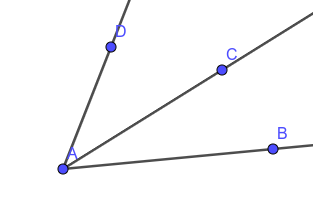
\includegraphics[width=2in]{geom-test1-review-img2.png}

\end{enumerate}
%\end{multicols}
\end{document}